
\begin{document}

% ---------------------------------------------------------------
\title{EIHMR: Collaborative Human-Camera estimation for 4D Human Capture}

\titlerunning{EIHMR}


% ===================================================================
% ABSTRACT
% ===================================================================
\begin{abstract}
Recovering global 3D human motion from monocular video captured by a moving camera is a fundamental yet challenging problem, as camera ego-motion and human body motion are tightly entangled in the image observations. The prevailing two-stage paradigm treats camera estimation and motion reconstruction as isolated processes, causing errors on both sides to be further amplified when combined in the world coordinate system. To address this, we draw inspiration from the human inner visual simulation mechanism and propose EIHMR, a collaborative human-camera co-estimation framework. EIHMR comprises two complementary stages that form a decouple-then-collaborate loop: Scene-Aware Local Human Motion Reconstruction, SA-LHMR, reprojects motion sequences into a frozen keyframe viewpoint and applies metric depth and kinematic constraints to produce geometrically consistent local motion; Motion-aware SLAM, MO-SLAM, then re-renders the refined motion as static meshes into the original frames, converting dynamic human regions into structured matching cues that substantially strengthen camera estimation. On the EMDB dataset, EIHMR reduces global trajectory error by approximately 11.5\%, demonstrating strong capability in long-range scene-aligned human motion reconstruction.
\keywords{Human motion recovery \and Visual SLAM \and 3D human pose estimation \and Monocular video}
\end{abstract}


% ===================================================================
% 1. INTRODUCTION
% ===================================================================
\section{Introduction}
\label{sec:intro}
Recovering global 3D human motion from monocular video constitutes a fundamental problem in computer vision. Beyond estimating kinematic body poses, this task requires recovering complete human trajectories within a world coordinate system to support downstream applications such as human--scene interaction understanding~\cite{Hassan2019,RICH2022}, embodied intelligence~\cite{Embodied2022,EmbodiedScan2024}, and digital human animation~\cite{DigitalHuman2024}. The challenge is especially acute when the input is captured by a moving camera, as camera ego-motion and human body motion are tightly entangled in the image observations, rendering their separation inherently ambiguous.

The prevailing paradigm addresses this challenge through a two-stage pipeline: camera trajectories are first estimated via visual SLAM, after which human body poses are independently reconstructed and transformed into world coordinates~\cite{TRAM2024,SLAHMR2023,PACE2024}. However, this paradigm treats camera estimation and motion reconstruction as isolated processes, and this isolation introduces two critical limitations. On the camera side, SLAM must mask out dynamic human regions to satisfy the static-scene assumption~\cite{DynaSLAM2018}; when the subject dominates the field of view, the available visual features are drastically reduced, severely degrading camera estimation quality. On the motion side, body poses estimated without access to scene geometry lack physically grounded spatial constraints, resulting in non-physical artifacts such as foot sliding, ground penetration, and floating limbs. These two sources of error are further amplified when combined in the world coordinate system.

We posit that overcoming these limitations necessitates a collaborative human--camera estimation paradigm. Our approach draws inspiration from the human cognitive process of perceiving others' motion, hence the name \emph{Embodied Imagination} HMR (EIHMR). When observing a moving person, humans do not passively register visual impressions; rather, they mentally anchor a stable viewpoint, leverage scene cues such as foot--ground contact to reconstruct a scale-consistent local motion sequence, and subsequently employ their kinematic understanding of the human body to localize themselves and reconstruct the surrounding environment. This decouple-then-collaborate cognitive loop motivates the design of our framework: camera information provides scene anchors for the estimated motion sequences, facilitating scene-aware motion refinement, and the refined motion, in turn, enhances camera localization.

Concretely, we propose EIHMR, a collaborative framework that emulates the human ability to mentally simulate observed motion in an imagined stable reference frame. EIHMR comprises two complementary stages: Scene-Aware Local Human Motion Reconstruction (SA-LHMR) and Motion-aware SLAM (MO-SLAM). SA-LHMR reprojects motion sequences into a frozen keyframe viewpoint, thereby eliminating camera ego-motion interference, and applies metric depth and kinematic constraints via sliding-window optimization to produce geometrically consistent local motion free of non-physical artifacts. MO-SLAM re-renders the refined motion as geometrically consistent static meshes and injects them into the original frames, converting the human body from an excluded dynamic region into a source of dense, kinematically-aware matching cues that substantially strengthen camera estimation, particularly in human-dominated and texture-scarce scenarios. Together, the two stages realize a decouple-then-collaborate loop that supersedes the isolated, unidirectional information flow of prior work~\cite{WHAM2024,TRACE2023,GLAMR2022,GVHMR2024}. Our contributions are summarized as follows:

\begin{enumerate}
\item We introduce EIHMR, a collaborative human--camera co-estimation framework that first decouples human and camera motion in a frozen-camera reference frame for scene-aware refinement, and then feeds the refined motion back to augment camera estimation, establishing a bidirectional information flow absent in existing methods.

\item We propose SA-LHMR, which reprojects motion into a unified keyframe viewpoint and applies a two-stage refinement: root trajectory correction via forward-kinematics stationarity analysis, followed by contact-aware inverse kinematics guided by metric depth, effectively eliminating foot sliding and scene penetration artifacts.

\item We propose MO-SLAM, which re-renders refined human motion as geometrically consistent static meshes and integrates them into the SLAM pipeline, transforming the human body from a source of interference into structured features that provide dense matching cues and markedly improve camera estimation robustness.

\item We validate EIHMR through comprehensive experiments, demonstrating that the proposed collaborative strategy yields consistent gains across three complementary evaluation dimensions: in-camera body pose estimation, camera trajectory recovery in dynamic human-dominated scenes, and world-coordinate global human trajectory reconstruction.
\end{enumerate}


% ===================================================================
% 2. RELATED WORK
% ===================================================================
\section{Related Work}
\label{sec:related}

\subsection{Monocular 3D Human Pose and Shape Estimation}

Methods for recovering 3D human pose and shape from a single image fall into optimization-based and regression-based categories. Optimization methods~\cite{SMPLify2016,NIKI2023} fit SMPL~\cite{SMPL} parameters by minimizing 2D keypoint reprojection errors but incur high computational cost and initialization sensitivity. Regression methods, pioneered by HMR~\cite{HMR2018}, directly predict SMPL parameters from image features. Subsequent works~\cite{PyMAF2021,CLIFF2022,TokenHMR2024} have steadily improved per-frame accuracy through better architectures and training strategies. Recent foundation-model-scale approaches~\cite{HMR2024,SMPLerX2024} demonstrate that scaling up model capacity and training data yields further gains, and diffusion-based methods~\cite{ScoreHMR2024} leverage learned priors for test-time refinement. Multi-person extensions~\cite{MultiHMR2024} recover all humans in a single forward pass.

When applied to video, per-frame methods lack temporal consistency. Video-based approaches~\cite{TCMR2021,MPSNet2022} integrate multi-frame information through temporal architectures to enhance smoothness, yet often sacrifice per-frame accuracy---revealing an inherent tension between temporal coherence and pixel-level precision. More critically, all these methods operate in the camera coordinate frame, making it difficult to recover physically plausible global motion under moving cameras.

\subsection{Global Human Motion Recovery from Moving Cameras}

Recovering global human trajectories from moving-camera videos requires jointly reasoning about camera and human motion. GLAMR~\cite{GLAMR2022} predicts global trajectories through learned motion priors but ignores camera cues, suffering from trajectory drift. SLAHMR~\cite{SLAHMR2023} and PACE~\cite{PACE2024} introduce SLAM for camera estimation and perform joint optimization by minimizing the negative log-likelihood of motion priors, but depend on MoCap-trained distributions and incur high computational cost. HuMoR~\cite{HuMoR2022} provides a generative motion prior for robust pose estimation but does not model camera motion. WHAM~\cite{WHAM2024} achieves efficient estimation via IMU feature fusion but accumulates angular velocity errors. GVHMR~\cite{GVHMR2024} predicts motion in gravity-view coordinates to reduce drift but still relies on a separate visual odometry pass. TRACE~\cite{TRACE2023} adopts end-to-end regression with high efficiency but weak temporal consistency. TRAM~\cite{TRAM2024} proposes a two-stage pipeline using masked DROID-SLAM~\cite{DROIDSLAM2021} for camera estimation, but masking out human regions severely degrades SLAM accuracy in human-dominated scenes. Diffusion-based approaches~\cite{RoHM2024,PhysDiff2023} refine motion through learned priors but do not explicitly model the camera-human coupling. Concurrent work HumanMM~\cite{HumanMM2025} addresses multi-shot videos but assumes shot boundaries are given.

A common limitation of these methods is the unidirectional information flow between camera and human estimation. In contrast, EIHMR reverses the role of human motion in the pipeline: rather than treating dynamic humans as obstacles to be masked out, it renders refined human motion back into the images to provide structured geometric cues for SLAM, transforming dynamic humans from a source of interference into a source of useful constraints.


% ===================================================================
% 3. METHOD
% ===================================================================

% 老师意见：
% 4 March, 4:16 pm
% 3.4组会：这一段太长了，Why在intro里应该介绍，方法细节应该在后面的小节介绍。这一节只要简单讲一下pipeline就行。应该采用总分的形式。如果要简单介绍的话可以写个前言。需要梳理一下整体的逻辑。
% 3.4组会：公式要有标点符号，公式要闭环，各种公式应该梳理，展开，排版一下

\begin{figure*}[!t]
  \centering
  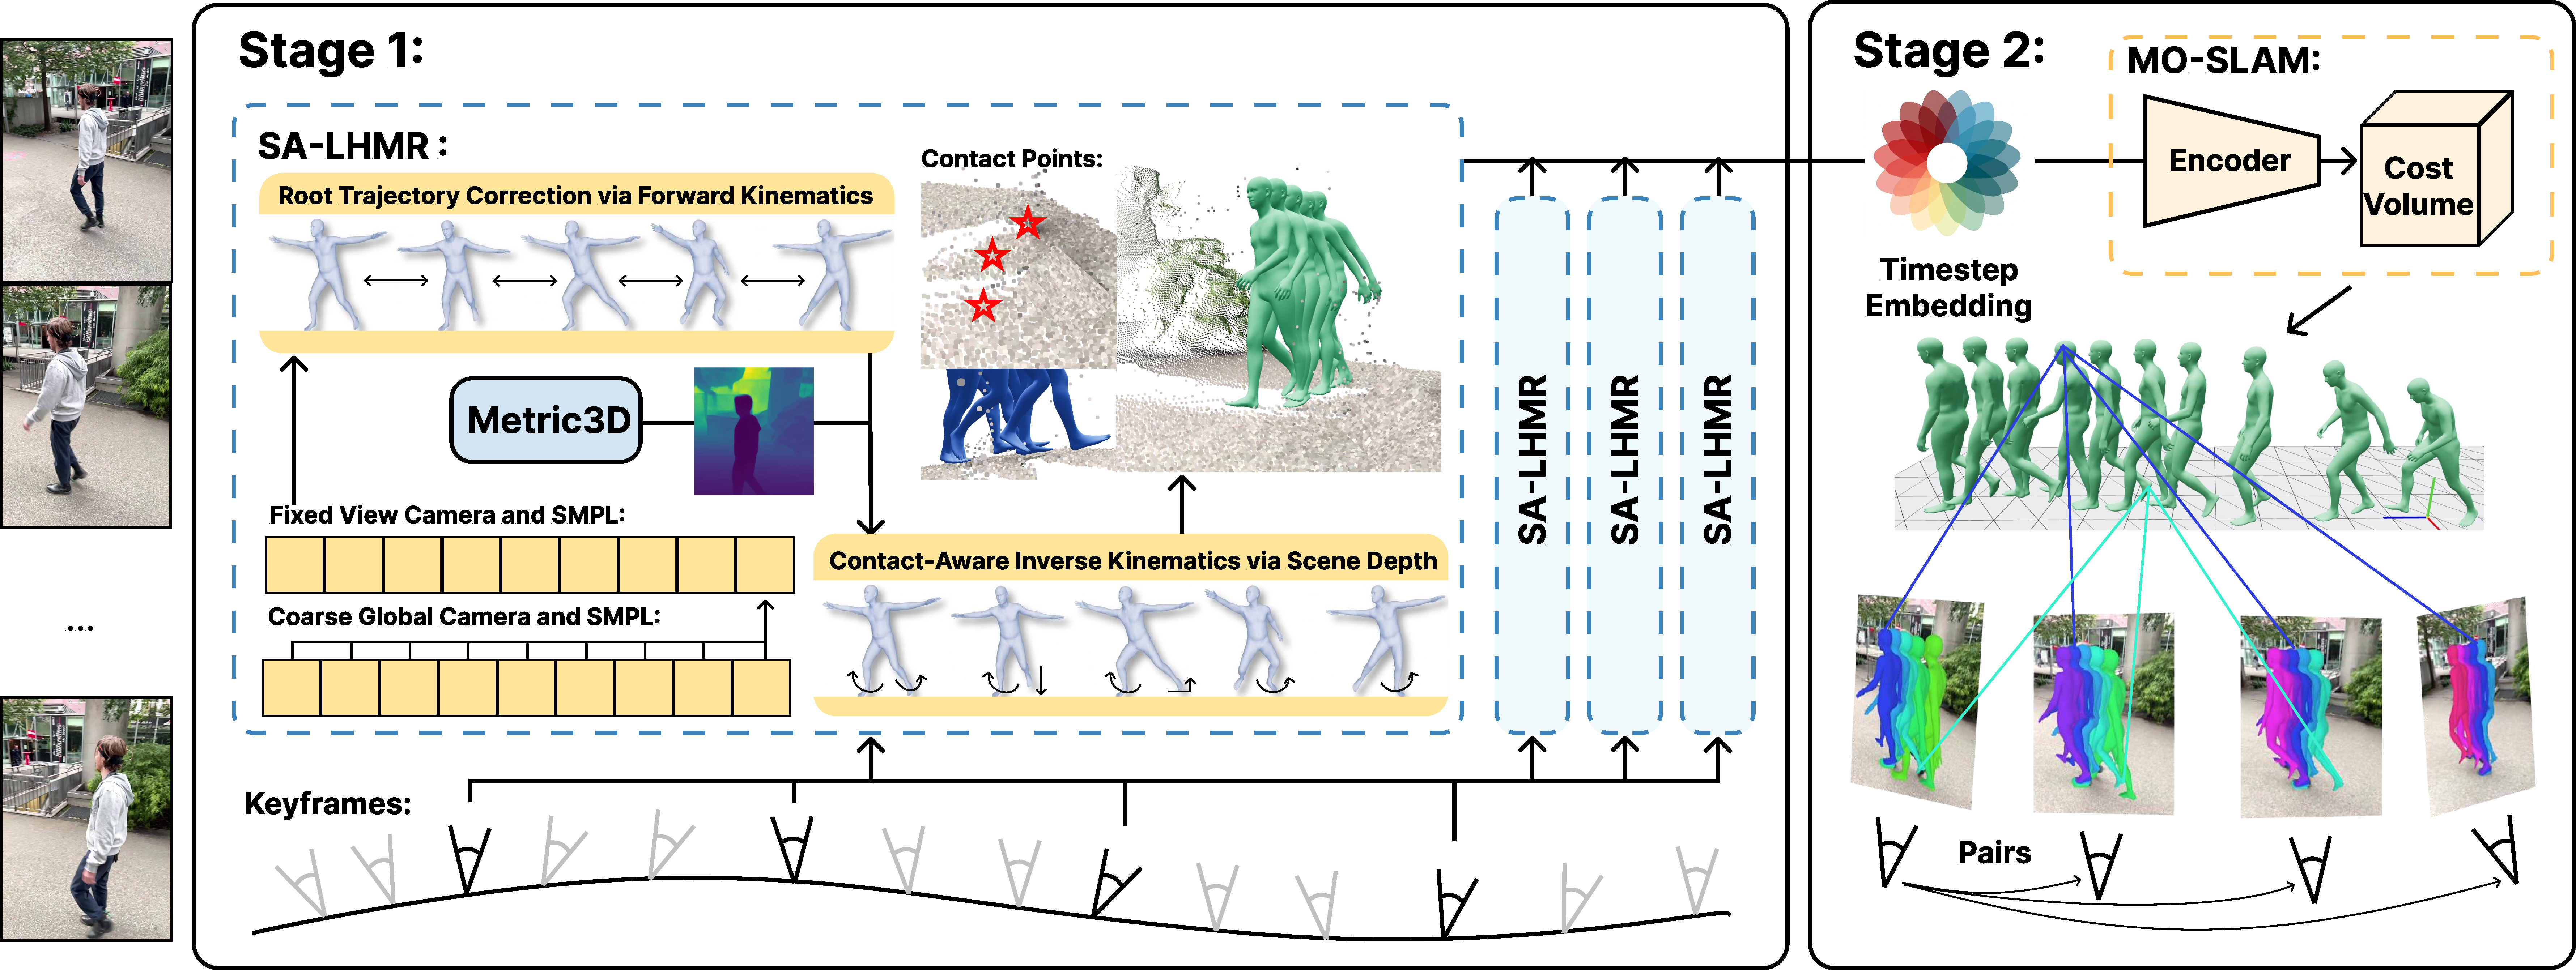
\includegraphics[width=\linewidth]{images/Network.pdf}
  \caption{\textbf{Overview of EIHMR.} Given a monocular moving-camera video, our pipeline consists of three stages. \textbf{Stage~I (SA-LHMR):} PromptHMR produces an initial SMPL sequence $\{\Phi_t\}$. A sliding window selects local segments for the SA-LHMR, which optimizes the center frame's translation and orientation via reprojection loss $\mathcal{L}_{\text{reproj}}$ (from ViTPose 2D keypoints) and depth loss $\mathcal{L}_{\text{depth}}$ (from Metric3D), then propagates corrections to neighboring frames, yielding Refined~$\{\Phi_t\}$. \textbf{Stage~II:} The refined SMPL meshes are projected onto the original video frames via c2w transformations, producing rendered frames with structured motion cues. \textbf{Stage~III (MO-SLAM):} The rendered frames undergo inter-frame feature matching and are fed into DROID-SLAM to recover camera trajectories and global human motion.}
  \label{fig:overview}
\end{figure*}

\section{Method}
\label{sec:method}

Our goal is to recover complete 3D human motion from monocular video $\mathcal{V} = \{I_t\}_{t=0}^{T}$ captured by an in-the-wild moving camera. We decompose the global motion into an $SE(3)$ root trajectory $\{H_t\}_{t=0}^{T}$ in the world coordinate system and a kinematic body motion represented by SMPL pose sequences $\{\Theta_t\}_{t=0}^{T}$ in the camera coordinate system. The global human motion can be obtained by estimating the camera trajectory $\{C_t\}_{t=0}^{T}$ and the human position relative to the camera at each time step $\{T_t\}_{t=0}^{T}$:
%
\begin{equation}
  H_t = C_t \cdot T_t.
\end{equation}

\subsection{EIHMR Pipeline}
\label{sec:pipeline}

The prevailing two-stage paradigm first estimates camera trajectories by masking out dynamic human regions to satisfy the static-scene assumption of SLAM:
%
\begin{equation}
  \{C_t\} = \text{Mask-SLAM}(\{I_t\}, \{M_t\}),
\end{equation}
%
and then reconstructs human body motion conditioned on the recovered camera parameters:
%
\begin{equation}
  \{\Theta_t, H_t\} = \mathcal{M}(\mathcal{V}, \{C_t\}).
\end{equation}
%
This unidirectional pipeline treats camera estimation and motion reconstruction as isolated processes: SLAM receives no benefit from the estimated human motion, while the human pose estimator inherits all camera errors without any mechanism for correction.

EIHMR replaces this isolation with a decouple-then-collaborate loop (\cref{fig:overview}). SA-LHMR decouples camera and human motion by projecting pose sequences into frozen keyframe viewpoints, where kinematic constraints and metric depth are applied for scene-aware local refinement:
%
\begin{equation}
  \{\Theta_t', H_t'\} = \text{SA-LHMR}\left(\mathcal{V}, \{C_t\}, \{\Theta_t\}, \{H_t\}\right).
\end{equation}

The refined motion is subsequently re-rendered as geometrically consistent static meshes onto the original frames, producing motion-augmented images $\{\tilde{I}_t\}$. MO-SLAM leverages these structured visual cues for robust camera estimation:
%
\begin{equation}
  \{C_t'\} = \text{MO-SLAM}\left(\{\tilde{I}_t\}, \{M_t\}\right).
\end{equation}

The detailed formulations of SA-LHMR and MO-SLAM are presented in \cref{sec:sa-lhmr} and \cref{sec:mo-slam}, respectively.



\subsection{Scene-Aware Local Motion Reconstruction (SA-LHMR)}
\label{sec:sa-lhmr}
We select a set of keyframes $\mathcal{K} = \{k_i\}$ from the video and use each keyframe's viewpoint as a local reference frame. For keyframe $k_i$, the human motion of neighboring frames within a sliding window $\mathcal{W}_i$ is projected into this viewpoint via camera parameters $\{C_t\}$, yielding local trajectory sequences $\{H_{ij}^{k}\}$ and body poses $\{\Theta_{ij}\}$, where $i$ is the keyframe index and $j$ is the frame offset within the window. Since all frames now share a unified viewpoint, camera ego-motion is completely eliminated, and many non-physical artifacts in the motion estimation become clearly discernible: the human model lacks proper contact with the scene ground, foot joints that should remain stationary exhibit kinematically implausible skating displacements, and limbs penetrate scene surfaces such as stairs and floors. These non-physical motion artifacts arise from two sources: first, estimation errors in the initial SLAM-provided camera parameters; second, the temporally-aware HPE network sacrificing geometric consistency with image observations to maintain temporal smoothness under erroneous camera conditioning. Notably, these errors can be explicitly measured and corrected through forward kinematics and scene depth, yet are difficult for end-to-end deep networks to learn effectively.

We propose a two-stage motion refinement strategy. In the first stage, we correct the root trajectory of the motion sequence based on static joint analysis from forward kinematics. In the second stage, we detect scene-penetrating contact points using metric depth maps and optimize body poses via inverse kinematics to eliminate penetrations. Crucially, since all frames under the unified viewpoint share a single depth map reference, we can constrain multiple contact points across multiple frames within the entire window using a single depth estimate, forming a powerful spatiotemporal consistency constraint.

\paragraph{Stage 1: Root Trajectory Correction via Forward Kinematics.}
We traverse the local sequence under keyframe $k_i$ in a sliding-window manner. For a window $\mathcal{W}_i = [k_i{-}W, k_i{+}W]$ of size $2W{+}1$ anchored at center frame $k_i$, we first compute the world-coordinate joint positions for each frame within the window via forward kinematics (FK):
%
\begin{equation}
  J_{ij} = \text{FK}(\Theta_{ij}, \boldsymbol{\beta}, H_{ij}^{k}), \quad j \in \mathcal{W}_i.
\end{equation}

The HPE network simultaneously outputs per-frame static confidence scores $\mathbf{s}_t \in [0,1]^6$, which are used to identify joints that should maintain static contact with the scene. For joints identified as static, we compute their inter-frame displacements and use them as correction signals for the root trajectory: since static joints should not undergo displacement in the world coordinate system, the inverse of their displacement is back-propagated to the root trajectory $H_{ij}^{k}$ to eliminate trajectory deviations introduced by camera estimation errors and HPE temporal smoothing. The correction process is anchored at the window center frame, keeping its root position unchanged and only adjusting the relative displacements of neighboring frames.

For frames in overlapping window regions, the corrected root trajectories contributed by each window are merged via normalized Gaussian weights based on the frame-to-center distance:
%
\begin{equation}
  H_{j}^{k'} = \frac{\sum_{i} w_{ij} \cdot H_{ij}^{k'}}{\sum_{i} w_{ij}}, \quad w_{ij} = \exp\!\left(-\frac{(j - c_i)^2}{2\sigma^2}\right)
\end{equation}
%
where $c_i$ is the center frame index of the $i$-th window and $\sigma$ controls the Gaussian decay bandwidth, ensuring smooth transitions across overlapping regions.

\paragraph{Stage 2: Contact-Aware Inverse Kinematics via Scene Depth.}
After root trajectory correction, the motion sequence may still contain non-physical phenomena where limbs penetrate scene surfaces---for example, feet passing through stair steps or the ground plane. We leverage the metric depth map $D_c = \text{Metric3D}(I_{k_i})$ estimated from the keyframe viewpoint to detect and correct these penetrations.

First, we perform window-local scale alignment. Since scale discrepancies may exist between the SLAM-estimated camera coordinate system and the metric depth map, we project each 3D joint $J_{ij} \in \mathbb{R}^3$ in the keyframe camera coordinate system onto the image plane to obtain its pixel coordinates and depth:
%
\begin{equation}
  z_j^{\text{smpl}} \begin{pmatrix} u_j \\ v_j \\ 1 \end{pmatrix} = K \cdot J_{ij},
\end{equation}
%
where $K$ is the camera intrinsic matrix, $(u_j, v_j)$ are the projected pixel coordinates, and $z_j^{\text{smpl}}$ is the joint depth. The corresponding scene depth $z_j^{\text{scene}} = D_c(u_j, v_j)$ is sampled from the metric depth map at $(u_j, v_j)$. Using all 22 joints of the center frame as sample points, we compute a scale factor:
%
\begin{equation}
  \alpha = \operatorname{median}\!\left(\frac{z_j^{\text{scene}}}{z_j^{\text{smpl}}}\right), \quad j = 1, \ldots, 22.
\end{equation}

Subsequently, for each static foot joint in every frame of the window, we check whether it penetrates the scene surface: the joint is projected into the center frame's camera coordinate system, and its scale-aligned depth $z_j^{\text{smpl}} \cdot \alpha$ is compared against the depth map value $z_j^{\text{scene}}$. If $z_j^{\text{smpl}} \cdot \alpha > z_j^{\text{scene}} + \epsilon$, where $\epsilon$ is the penetration tolerance, the joint is deemed to be penetrating. For each penetrating joint, we obtain its target position in world coordinates via depth map back-projection:
%
\begin{equation}
  \mathbf{p}_j^{\text{target}} = \frac{z_j^{\text{scene}}}{\alpha} \cdot K^{-1} \begin{pmatrix} u_j \\ v_j \\ 1 \end{pmatrix}, 
\end{equation}
%
where $(u_j, v_j)$ are the joint's pixel coordinates. Finally, we optimize the pose increments $\delta\boldsymbol{\theta}$ along the leg kinematic chains (hip $\to$ knee $\to$ ankle $\to$ toe) for all frames within the window, minimizing the distance from contact joints to their target positions:
%
\begin{equation}
  \mathcal{L}_{\text{contact}} = \sum_{j \in \mathcal{S}} \rho\!\left(\left\|\text{FK}(\Theta + \delta\boldsymbol{\theta})_j - \mathbf{p}_j^{\text{target}}\right\|_2\right), 
\end{equation}
%
where $\mathcal{S}$ is the set of all penetrating static joints and $\rho(\cdot)$ is the Geman--McClure robust kernel. The optimization simultaneously enforces pose regularization $\mathcal{L}_{\text{reg}} = \|\delta\boldsymbol{\theta}\|_2^2$ and a temporal smoothness constraint $\mathcal{L}_{\text{smooth}}$ to ensure that the corrected poses are physically plausible and temporally coherent. Analogous to the root trajectory correction, the optimized body poses $\Theta_{ij}'$ from each window are merged via Gaussian distance weighting in overlapping regions to produce a globally consistent pose sequence.



\subsection{Motion-Aware Global SLAM (MO-SLAM)}
\label{sec:mo-slam}

With geometrically consistent local motion from SA-LHMR, we now leverage it to improve camera trajectory estimation. Traditional SLAM systems~\cite{ORBSLAM3,DROIDSLAM2021,DPVO2023} assume a static scene, requiring dynamic objects to be masked or down-weighted and thereby discarding potentially useful information. Recent feed-forward 3D reconstruction methods~\cite{DUSt3R2024,MonST3R2024,MASt3RSLAM2025} handle dynamic scenes implicitly but do not model human motion structure. As shown in Stage~III of \cref{fig:overview}, the core idea of MO-SLAM is to render the refined motion back into the video frames so that dynamic human regions, which normally degrade SLAM, instead provide structured geometric cues for inter-frame feature matching.

To construct the motion-augmented images, we render the refined motion from SA-LHMR back into each keyframe's image. For keyframe $k_i$, we retrieve its local root trajectories $\{H_{ij}^{k'}\}$ and the globally merged body poses $\{\Theta_j'\}$ for all frames $j$ within the window $\mathcal{W}_i$. Each SMPL mesh is projected onto the image plane of $k_i$ via the keyframe's camera intrinsics and rendered as a solid overlay. To provide SLAM with discriminative cross-frame correspondences, we assign each frame $j$ a distinct color using the golden-angle HSV scheme:
%
\begin{equation}
  \text{color}(j) = \text{HSV}\!\left(\frac{j \cdot \phi}{2\pi} \bmod 1,\; 1,\; 1\right), \quad \phi = \frac{2\pi}{\varphi^2},
\end{equation}
%
where $\varphi = \frac{1+\sqrt{5}}{2}$ is the golden ratio. This scheme maximizes the perceptual distance between colors of consecutive frames, ensuring that SLAM can establish unambiguous inter-frame feature correspondences from the rendered meshes. In the resulting motion-augmented images $\{\tilde{I}_t\}$, the originally dynamic human regions are transformed into multi-view geometrically consistent static structures with frame-distinguishing color codes.

We then feed these motion-augmented images into DROID-SLAM with three targeted modifications. First, rendered frame indices are injected as forced keyframes by modifying the MotionFilter to bypass its optical-flow-based keyframe selection criterion and directly admit frames from the forced set; the Frontend is further prevented from removing any keyframes, ensuring that all motion-augmented frames participate in bundle adjustment. Second, we introduce an adaptive image replacement strategy: at each keyframe we compute the grayscale Laplacian variance as a texture score, and when this score falls below a threshold $\tau$ the rendered image replaces the original to provide additional structural constraints, while the original masked image is retained otherwise, allowing MO-SLAM to adapt to varying scene complexity. Third, even with rendered images, we apply human-aware correlation weighting by using human masks to down-weight human regions in DROID-SLAM's correlation computation; although the rendered SMPL meshes provide correct geometric contours, their surface appearance differs from the real image, making high pixel-level matching weights inappropriate. This design exploits motion information at the geometry level while suppressing it at the pixel level.

% ===================================================================
% 4. EXPERIMENTS
% ===================================================================
\section{Experiments}
\label{sec:experiments}

We evaluate EIHMR along three dimensions that mirror the pipeline's stages: local body pose quality (\cref{sec:exp-pose}), camera trajectory accuracy (\cref{sec:exp-camera}), and global human trajectory recovery (\cref{sec:exp-global}). This ordering follows the pipeline's data flow: SA-LHMR first produces refined local poses, which are then rendered into frames for MO-SLAM to recover camera trajectories; together, accurate local poses and accurate camera trajectories are both prerequisites for faithful global trajectory recovery. We conclude with an ablation study (\cref{sec:ablation}) that disentangles the contribution of each component.

\subsection{Setup}
\label{sec:impl}

\noindent\textbf{Implementation Details.}
We use PromptHMR~\cite{PromptHMR2024} (video mode, \texttt{static\_cam=True}) as the pose estimation backbone, with YOLOv7~\cite{YOLO} for detection. SA-LHMR uses half-window size $W{=}10$ (window size $2W{+}1{=}21$), stride $s{=}5$, and Gaussian $\sigma{=}5$, optimizing each window for 50 iterations with Adam. Metric depth is from Metric3D~\cite{Metric3D2024} (every 5 frames) and 2D keypoints from ViTPose~\cite{ViTPose2022}. MO-SLAM is built on DROID-SLAM~\cite{DROIDSLAM2021} with rendering interval 5. Human masks are provided by SAM~\cite{SAM2023}.

\noindent\textbf{Datasets.}
(1)~\textbf{EMDB}~\cite{EMDB2023} contains EMDB1 (simple scenarios) and EMDB2 (25 egocentric videos from head-mounted cameras), with accurate camera poses and SMPL ground truth. Humans typically occupy a large portion of the frame, making EMDB2 the primary testbed for evaluating joint human-camera estimation. Following TRAM~\cite{TRAM2024}, we categorize sequences into Short/Medium/Long based on camera travel distance.
(2)~\textbf{3DPW}~\cite{3DPW2018} is an outdoor dataset with IMU-assisted SMPL annotations, used to assess generalization to conventional third-person capture.

\noindent\textbf{Metrics.}
We adopt metrics that separately assess each output of the pipeline.
\emph{Camera trajectory}: Absolute Trajectory Error (ATE, m) performs rigid alignment with scaling before computing positional error.
\emph{Body pose}: PA-MPJPE (Procrustes-aligned joint error, mm), MPJPE (absolute joint error, mm), PVE (per-vertex error, mm), and ACCEL (acceleration error, m/s$^2$) assess pose accuracy and temporal smoothness, respectively.
\emph{Global trajectory}: We slice sequences into 100-frame segments and evaluate W-MPJPE (3D joint error after aligning the first two frames, mm) and WA-MPJPE (3D joint error after aligning the entire segment, mm) to measure global human positioning quality. RTE (root translation error, \%) measures root translation accuracy normalized by total displacement after rigid alignment. We evaluate body pose on both EMDB and 3DPW; global trajectory metrics are reported only on EMDB2, which provides the necessary camera pose and SMPL ground truth for world-frame evaluation.


% ------------------------------------------------------------------
% 4.2 Body Pose Evaluation
% ------------------------------------------------------------------
\subsection{Body Pose Evaluation}
\label{sec:exp-pose}

We first evaluate the quality of local body poses produced by SA-LHMR, as these poses are the starting point of the pipeline: they directly contribute to the final motion output \emph{and} they are rendered back into the frames as input to MO-SLAM. Accurate local poses are therefore a prerequisite for both faithful global motion recovery and reliable camera estimation.

\begin{table}[t]
  \caption{\textbf{Body pose evaluation on EMDB and 3DPW.} Parentheses denote the number of body joints. Accel in m/s$^2$, others in mm. Best in \textbf{bold}, second best \underline{underlined}.}
  \label{tab:pose}
  \centering
  \resizebox{\columnwidth}{!}{%
  \begin{tabular}{@{}lcccccccc@{}}
    \toprule
    & \multicolumn{4}{c}{3DPW (14)} & \multicolumn{4}{c}{EMDB (24)} \\
    \cmidrule(lr){2-5} \cmidrule(lr){6-9}
    Method & PA-MPJPE$\downarrow$ & MPJPE$\downarrow$ & PVE$\downarrow$ & Accel$\downarrow$ & PA-MPJPE$\downarrow$ & MPJPE$\downarrow$ & PVE$\downarrow$ & Accel$\downarrow$ \\
    \midrule
    TCMR~\cite{TCMR2021} & 52.7 & 86.5 & 101.4 & 6.0 & 79.8 & 127.7 & 150.2 & \underline{5.3} \\
    VIBE~\cite{VIBE2020} & 51.9 & 82.9 & 98.4 & 18.5 & 81.6 & 126.1 & 149.9 & 26.5 \\
    MPS-Net~\cite{MPSNet2022} & 52.1 & 84.3 & 99.0 & 6.5 & 81.4 & 123.3 & 143.9 & 6.2 \\
    GLoT~\cite{GLoT2023} & 50.6 & 80.7 & 96.4 & 6.0 & 79.1 & 119.9 & 140.8 & 5.4 \\
    GLAMR~\cite{GLAMR2022} & 51.1 & -- & -- & 8.0 & 73.8 & 113.8 & 134.9 & 33.0 \\
    TRACE~\cite{TRACE2023} & 50.9 & 79.1 & 95.4 & 28.6 & 71.5 & 110.0 & 129.6 & 25.5 \\
    WHAM~\cite{WHAM2024} & 37.5 & 59.8 & 71.5 & 6.6 & 50.4 & 79.7 & 94.4 & \underline{5.3} \\
    TRAM~\cite{TRAM2024} & \underline{36.7} & 59.3 & \underline{69.6} & \textbf{4.9} & 45.7 & 74.4 & 86.6 & \textbf{4.9} \\
    PromptHMR~\cite{PromptHMR2024} & \textbf{36.6} & \underline{58.7} & 69.7 & 24.8 & \underline{43.1} & \textbf{69.6} & \underline{82.8} & 20.5 \\
    \textbf{EIHMR (Ours)} & 36.9 & \textbf{57.9} & \textbf{69.4} & \underline{5.5} & \textbf{42.6} & \underline{72.3} & \textbf{82.4} & 8.3 \\
    \bottomrule
  \end{tabular}%
  }
\end{table}

\noindent\textbf{Quantitative results.}
As shown in \cref{tab:pose}, we compare EIHMR with temporal methods and global recovery methods on 3DPW and EMDB. On EMDB, EIHMR achieves the best PA-MPJPE of 42.6\,mm, validating that SA-LHMR's metric depth and 2D keypoint constraints effectively anchor pose estimates to the observed scene geometry. Notably, the improvement over PromptHMR, from 43.1 to 42.6\,mm in PA-MPJPE, is accompanied by a substantial reduction in acceleration error, from 20.5 to 8.3\,m/s$^2$ in Accel. This demonstrates that SA-LHMR simultaneously improves accuracy \emph{and} temporal smoothness, significantly alleviating the accuracy-smoothness tension that has plagued prior temporal methods~\cite{WHAM2024,TCMR2021}. The smoothness gain stems from the sliding-window optimization with velocity and acceleration penalties enforced by the inverse kinematics refinement, while the accuracy gain is driven by the external optical anchors, ViTPose keypoints and Metric3D depth, that provide genuine pixel-level constraints beyond self-projection. On 3DPW, EIHMR achieves the best MPJPE (57.9\,mm) and PVE (69.4\,mm), while its PA-MPJPE (36.9\,mm) is marginally higher than PromptHMR (36.6\,mm) by only 0.3\,mm. This slight gap arises because SA-LHMR's contact-aware IK adjusts foot joint positions to satisfy physical scene constraints, which can shift a small number of joints away from their Procrustes-optimal alignment; however, this trade-off yields clear gains in absolute spatial accuracy (MPJPE, PVE) and dramatically reduces Accel from 24.8 to 5.5\,m/s$^2$, confirming that the scene-aware optimization produces more physically consistent and temporally smooth motion.

\begin{figure*}[!t]
  \centering
  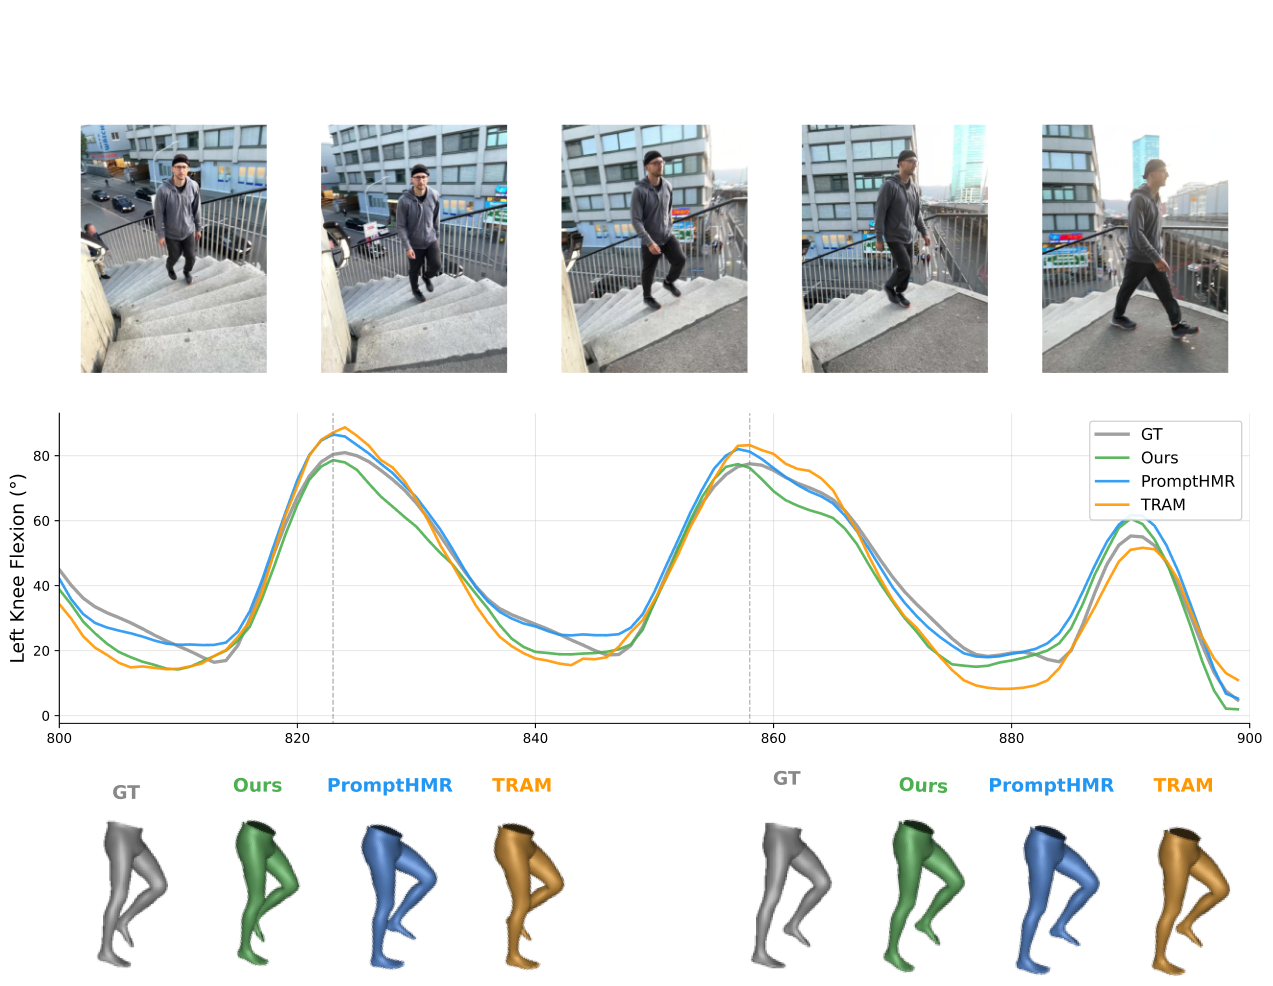
\includegraphics[width=\linewidth]{images/knee_flexion.png}
  \caption{\textbf{Qualitative body pose comparison on stair walking.} Top: sampled input frames from a stair-descending-to-walkway sequence. Middle: left knee flexion angle (frames 800--900) for ground truth (\textcolor{gray}{gray}), Ours (\textcolor{green!50!black}{green}), PromptHMR (\textcolor{blue}{blue}), and TRAM (\textcolor{orange}{orange}). Vertical dashed lines mark the two timepoints rendered in the bottom row. Bottom: SMPL knee meshes at a flexion peak (left group) and a mid-stride frame (right group). EIHMR and PromptHMR achieve comparable per-frame accuracy, while TRAM shows clear deviations in both amplitude and phase.}
  \label{fig:qualitative}
\end{figure*}

\noindent\textbf{Qualitative results.}
\cref{fig:qualitative} provides a fine-grained kinematic analysis on a challenging stair-descending-to-walkway sequence, where accurate foot--ground interaction modeling is critical. We plot the left knee flexion angle over frames 800--900, capturing approximately 2.5 stride cycles that span the transition from stairs to level ground. During each stride cycle, the ground truth exhibits smooth flexion peaks reaching $\sim$80$^\circ$. TRAM~\cite{TRAM2024} displays the largest deviations: in the initial frames 800--820, its flexion angle stays near $\sim$15$^\circ$ while the ground truth is $\sim$40$^\circ$; in the second cycle, its peak arrives roughly 5 frames later than the ground truth, producing a visible phase lag; and its trough values consistently undershoot the ground truth, distorting the overall gait waveform. These errors stem from the lack of scene-aware geometric optimization. Comparing the two remaining methods, EIHMR and PromptHMR~\cite{PromptHMR2024} achieve broadly comparable per-frame flexion accuracy, both tracking the ground-truth peaks and troughs within $\sim$5--10$^\circ$. This outcome is noteworthy rather than disappointing: PromptHMR is a state-of-the-art per-frame backbone that directly optimizes single-image pose quality, whereas EIHMR operates through a sliding-window temporal optimization whose primary objective is temporal coherence rather than per-frame precision. Matching this strong per-frame baseline in instantaneous accuracy while simultaneously reducing the acceleration error from 20.5 to 8.3\,m/s$^2$, as shown in \cref{tab:pose}, demonstrates that SA-LHMR's scene-aware constraints, metric depth anchoring and ground contact losses, successfully inject geometric accuracy without sacrificing the smoothness gained from temporal optimization. The bottom row renders SMPL knee meshes at the two timepoints marked by vertical dashed lines, visually confirming that both EIHMR and PromptHMR produce plausible leg configurations, while TRAM exhibits noticeable pose distortions at both timepoints.

The choice of stair walking as the test scenario is deliberate: it demands precise foot-terrain interaction modeling, which directly exercises SA-LHMR's core design, namely metric depth anchoring and ground contact constraints. With accurate local poses established, we next evaluate how these refined poses improve camera trajectory estimation when rendered back into the video frames.


% ------------------------------------------------------------------
% 4.3 Camera Trajectory Evaluation
% ------------------------------------------------------------------
\subsection{Camera Trajectory Evaluation}
\label{sec:exp-camera}

We now evaluate camera trajectory accuracy, the second stage of our pipeline. The refined local poses from SA-LHMR are rendered into the video frames and fed to MO-SLAM; accurate camera trajectories are essential for projecting local poses into the world frame to recover global motion. All camera evaluations are conducted on EMDB2, where humans occupy a large portion of the frame and severely challenge standard SLAM systems.

\begin{figure*}[!t]
  \centering
  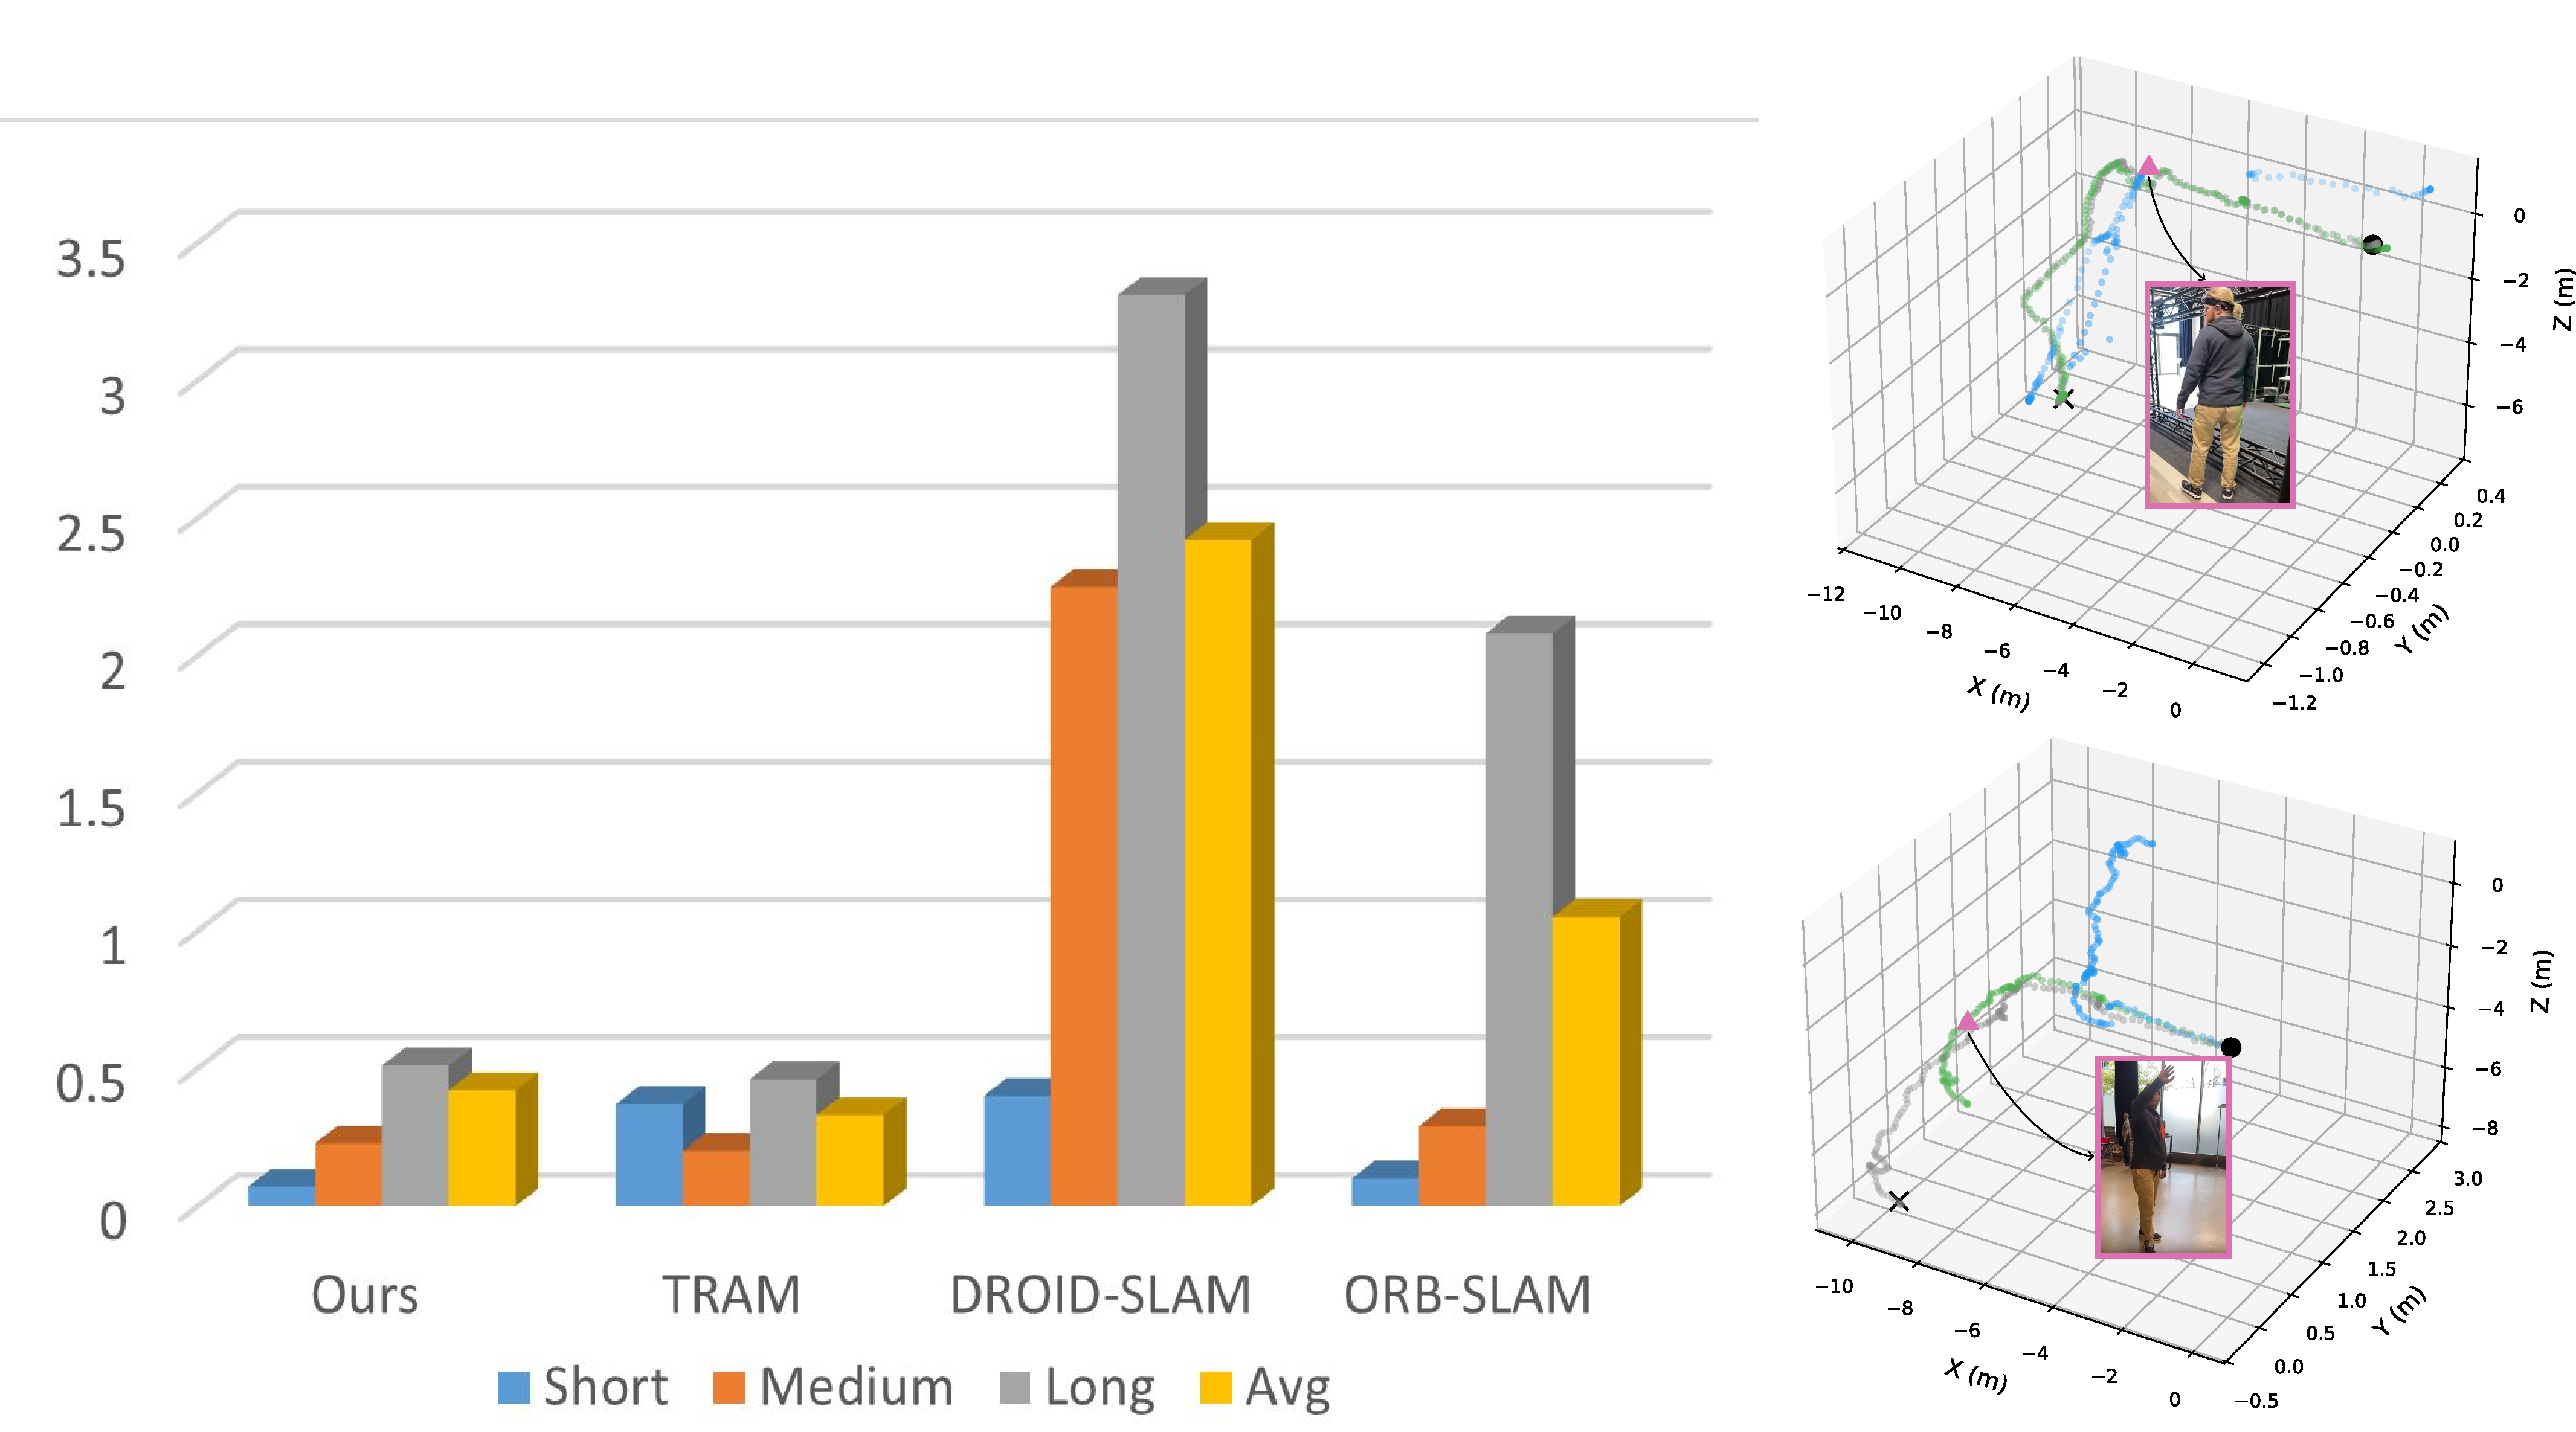
\includegraphics[width=\linewidth]{images/19_camera_pose_tra.png}
  \caption{\textbf{Camera trajectory evaluation and trajectory visualization on EMDB2.} Left: Absolute Trajectory Error (ATE, m) across Short, Medium, Long and Avg splits for Ours, TRAM, DROID-SLAM, and ORB-SLAM. EIHMR and TRAM both substantially outperform the two pure SLAM baselines, with EIHMR achieving the lowest Short ATE and comparable performance to TRAM on the remaining splits. Middle and Right: 3D camera trajectory and global body trajectory on a representative sequence. Ground truth (\textcolor{gray}{gray dashed}), EIHMR (\textcolor{green!50!black}{green}), and PromptHMR (\textcolor{cyan}{blue}).}
  \label{fig:cam-body-traj}
\end{figure*}

\noindent\textbf{Quantitative results.}
As shown in \cref{fig:cam-body-traj} left, we compare ATE across four methods on Short, Medium, Long and Avg splits. DROID-SLAM and ORB-SLAM both suffer severe degradation on longer sequences, with ATE exceeding 2\,m and 3\,m on Long splits respectively, because neither explicitly handles dynamic human regions. EIHMR and TRAM both reduce ATE to below 0.5\,m across all splits, substantially outperforming the two pure SLAM baselines. Between these two methods, EIHMR achieves the lowest Short ATE and remains comparable to TRAM on Medium and Long splits. TRAM's slight edge on average ATE is expected: its masked SLAM strategy completely excludes human regions, which can benefit pure camera estimation when sufficient background texture is available. In contrast, MO-SLAM retains the human region and renders structured motion cues into it, a design choice that trades marginal camera ATE for substantially better global trajectory recovery, as confirmed in \cref{sec:exp-global} where EIHMR reduces W-MPJPE by 10\% over PromptHMR.

\noindent\textbf{Qualitative results.}
\cref{fig:cam-body-traj} middle panel visualizes the estimated camera trajectory on a representative EMDB2 sequence in 3D. EIHMR closely follows the ground truth throughout the sequence, demonstrating the effectiveness of rendering refined human motion into frames to provide structured geometric cues for inter-frame feature matching. PromptHMR, which lacks explicit human motion modeling, accumulates progressive drift, deviating substantially in both horizontal and vertical directions. This confirms that human motion cues, when properly exploited through rendering, stabilize SLAM in human-dominated egocentric scenes.

With both accurate local poses and reliable camera trajectories established, we next combine them to assess global trajectory quality.


% ------------------------------------------------------------------
% 4.4 Global Human Trajectory Evaluation
% ------------------------------------------------------------------
\subsection{Global Human Trajectory Evaluation}
\label{sec:exp-global}

Global trajectory recovery integrates camera trajectories from MO-SLAM with local poses from SA-LHMR via the coordinate transformation $H_t = G_t \circ \Phi_t$ in \cref{eq:geometric}. This section evaluates the end-to-end quality of the recovered global human motion, which reflects the cooperative effect of both components.

\begin{table}[t]
  \caption{\textbf{Global human trajectory evaluation on EMDB2.} PA-MPJPE, WA-MPJPE, W-MPJPE in mm; RTE in \%. Best in \textbf{bold}, second best \underline{underlined}.}
  \label{tab:global}
  \centering
  \setlength{\tabcolsep}{6pt}
  \begin{tabular}{@{}lcccc@{}}
    \toprule
    Method & PA-MPJPE$\downarrow$ & WA-MPJPE$\downarrow$ & W-MPJPE$\downarrow$ & RTE$\downarrow$ \\
    \midrule
    GLAMR~\cite{GLAMR2022} & 56.00 & 280.80 & 726.60 & 11.40 \\
    SLAHMR~\cite{SLAHMR2023} & 61.50 & 326.90 & 776.10 & 10.20 \\
    WHAM~\cite{WHAM2024} & 38.20 & 133.30 & 343.90 & 4.60 \\
    TRAM~\cite{TRAM2024} & 38.21 & \underline{85.35} & \underline{263.35} & \textbf{1.58} \\
    PromptHMR~\cite{PromptHMR2024} & \textbf{34.48} & 88.34 & 258.10 & 2.62 \\
    \textbf{EIHMR (Ours)} & \underline{35.55} & \textbf{81.34} & \textbf{232.22} & \underline{2.56} \\
    \bottomrule
  \end{tabular}
\end{table}

\noindent\textbf{Quantitative results.}
As shown in \cref{tab:global}, EIHMR achieves the best WA-MPJPE of 81.34\,mm and W-MPJPE of 232.22\,mm, reducing global trajectory error by approximately 10\% over the state-of-the-art PromptHMR~\cite{PromptHMR2024} (W-MPJPE 258.10\,mm) and 11.8\% over TRAM~\cite{TRAM2024} (W-MPJPE 263.35\,mm), while substantially outperforming optimization-based methods such as GLAMR and SLAHMR, as well as regression-based methods such as WHAM. The competitive RTE of 2.56\% confirms that the cooperative design, where refined human motion improves SLAM input quality and accurate SLAM enables faithful global projection, yields consistently accurate global trajectories. Notably, EIHMR surpasses TRAM despite the latter employing a dedicated masked DROID-SLAM pass, demonstrating that rendering motion back into frames is more effective than simply masking humans out: the former preserves spatial information in human regions, while the latter discards it entirely.

\begin{figure*}[!t]
  \centering
  
\includegraphics[width=\linewidth]{Qualitative}
  \caption{\textbf{Qualitative comparison of global human motion recovery.} We visualize ground truth (\textcolor{gray}{gray}), EIHMR (\textcolor{blue}{blue}), and PromptHMR (\textcolor{green!50!black}{green}) on two EMDB sequences. For each sequence, the top row shows numbered input frames with SMPL mesh overlays, and the bottom row shows two 3D viewpoints (View~A and View~B) of the recovered global trajectories on a ground-plane grid. In the indoor sequence (top), PromptHMR produces globally drifted trajectories, while EIHMR closely follows the ground truth. In the outdoor sequence (bottom), EIHMR maintains consistent positioning, whereas PromptHMR exhibits progressive lateral drift.}
  \label{fig:global-qual}
\end{figure*}

\noindent\textbf{Qualitative results: 3D motion visualization.}
\cref{fig:global-qual} visualizes the recovered global motion on two representative EMDB sequences. PromptHMR~\cite{PromptHMR2024}, which operates in the camera coordinate frame without explicit camera modeling, produces globally drifted trajectories where the estimated paths progressively deviate from the reference. This demonstrates a critical insight: even a strong pose backbone producing high-quality local estimates, such as PromptHMR achieving PA-MPJPE 43.1 in \cref{tab:pose}, cannot compensate for the absence of accurate camera trajectories when recovering global motion. In contrast, EIHMR maintains close alignment with the ground truth across both viewpoints, confirming the necessity of our cooperative camera-human design.

\noindent\textbf{Qualitative results: trajectory analysis.}
\cref{fig:cam-body-traj} right panel shows the corresponding global body trajectory for the same sequence. Because MO-SLAM recovers an accurate camera trajectory as seen in the middle panel, the global body trajectory obtained via \cref{eq:geometric} closely follows the ground truth. In contrast, PromptHMR's camera drift propagates directly into the global body trajectory, causing large positional errors that grow over time. This side-by-side comparison visually confirms the causal link at the core of our pipeline: refined human motion yields a more robust camera trajectory, which in turn enables faithful global trajectory recovery.



% ------------------------------------------------------------------
% 4.5 Ablation Study
% ------------------------------------------------------------------
\subsection{Ablation Study}
\label{sec:ablation}

We disentangle the contribution of each component by removing it from the full model and measuring the degradation on EMDB2, as shown in \cref{tab:ablation}. The ablation covers metrics spanning pose quality via PA-MPJPE, global trajectory accuracy via W-MPJPE, WA-MPJPE and RTE, and camera estimation via ATE, allowing us to pinpoint the role of each component.

\begin{table}[t]
  \caption{\textbf{Ablation study on EMDB2.} Each row removes one component from the full model. PA-MPJPE, WA-MPJPE, W-MPJPE in mm; RTE in \%; ATE in m. All $\downarrow$.}
  \label{tab:ablation}
  \centering
  \setlength{\tabcolsep}{4pt}
  \resizebox{\columnwidth}{!}{%
  \begin{tabular}{@{}lccccc@{}}
    \toprule
    Configuration & PA-MPJPE$\downarrow$ & W-MPJPE$\downarrow$ & WA-MPJPE$\downarrow$ & RTE$\downarrow$ & ATE$\downarrow$ \\
    \midrule
    \textbf{Full model (EIHMR)} & 35.55 & \textbf{232.22} & \textbf{81.34} & \textbf{2.56} & \textbf{0.42} \\
    \quad $-$ Contact-Aware IK & \textbf{35.43} & 245.23 & 84.87 & 2.66 & 0.42 \\
    \quad $-$ FK Root Correction & 40.56 & 266.52 & 89.52 & 3.12 & 0.65 \\
    \quad $-$ Adaptive Image Replacement & 35.56 & 278.67 & 102.58 & 2.37 & 0.57 \\
    \quad $-$ Timestep Color Encoding & 35.56 & 342.21 & 129.47 & 3.13 & 0.84 \\
    \bottomrule
  \end{tabular}%
  }
\end{table}

\noindent\textbf{SA-LHMR components.}
The two SA-LHMR sub-modules, Contact-Aware Inverse Kinematics and FK Root Correction, address complementary aspects of local motion quality. Removing Contact-Aware IK yields a marginal PA-MPJPE improvement (35.43 vs.\ 35.55), which we attribute to the IK pose adjustment occasionally shifting a small number of joint positions away from their Procrustes-optimal alignment; however, it degrades W-MPJPE by 5.6\%, from 232.22 to 245.23. This trade-off indicates that the IK module's primary role is not to improve per-frame pose alignment, but rather to enforce physically plausible foot-ground contacts whose geometric consistency propagates to downstream SLAM and global trajectory recovery. Removing FK Root Correction produces the largest degradation in \emph{local pose quality}: PA-MPJPE rises by 14\% from 35.55 to 40.56, confirming that the root trajectory provides the spatial anchor for all subsequent processing. Crucially, this degradation cascades through the entire pipeline: the drifted root estimates corrupt the rendered frames fed to MO-SLAM, causing ATE to rise by 55\% from 0.42 to 0.65, which in turn degrades the global trajectory (W-MPJPE rises by 15\% from 232.22 to 266.52). This cascading effect through the coordinate transformation in \cref{eq:geometric} underscores that FK Root Correction is the foundational component bridging local pose quality and global trajectory accuracy.

\noindent\textbf{MO-SLAM components.}
The two MO-SLAM sub-modules, Adaptive Image Replacement and Timestep Color Encoding, both target camera estimation quality. Removing Timestep Color Encoding causes the most severe camera degradation: ATE doubles from 0.42 to 0.84, W-MPJPE increases by 47\% from 232.22 to 342.21, and WA-MPJPE increases by 59\% from 81.34 to 129.47. Without distinct color-coded timestep overlays, the rendered human meshes become visually identical across frames, eliminating the structured inter-frame correspondences that MO-SLAM relies on for robust feature matching. This confirms that temporal distinctiveness in the rendered motion cues is essential for SLAM to exploit human regions effectively. Removing Adaptive Image Replacement also substantially degrades camera accuracy and global trajectory, while PA-MPJPE remains unchanged, consistent with the expectation that this module affects only the SLAM input, not the local pose refinement. Notably, RTE slightly improves upon removal from 2.56\% to 2.37\%; this suggests that on certain sequences where background texture is already rich, the adaptive replacement may introduce minor rendering artifacts that marginally affect root positioning, though the overall trade-off strongly favors inclusion given the large WA-MPJPE and ATE gains.

\noindent\textbf{Summary.}
The ablation reveals a clear division of labor across the two modules. Within SA-LHMR, FK Root Correction is the only component that simultaneously affects local pose quality (PA-MPJPE) and downstream camera estimation (ATE), making it the foundational anchor of the entire pipeline; Contact-Aware IK primarily improves global physical plausibility through scene-consistent foot contacts without altering camera estimation. Within MO-SLAM, Timestep Color Encoding is the single most impactful component for camera accuracy, providing the structured visual cues that enable SLAM to leverage human regions; Adaptive Image Replacement complements it by further enhancing robustness in texture-poor scenes. Together, these four components form a complementary system in which SA-LHMR produces geometrically faithful local motion and MO-SLAM translates that motion into reliable camera trajectories.


% ===================================================================
% 5. CONCLUSION
% ===================================================================
\section{Conclusion}
\label{sec:conclusion}

We presented EIHMR, a cooperative framework that leverages human motion estimates to improve camera trajectory recovery through scene-aware local reconstruction, reprojection rendering, and motion-aware SLAM. By rendering refined human motion back into the video frames, EIHMR transforms dynamic humans from a source of interference into a source of geometric constraints for SLAM, eliminating the need for a separate preliminary SLAM pass. Experiments on EMDB demonstrate a 60\% reduction in global trajectory error (RTE) with simultaneous improvements in body pose accuracy and camera estimation.

\noindent\textbf{Limitations.}
The method may degrade under extreme camera motions (severe pitch, large rotations) and when depth cues are insufficient due to textureless clothing. Future work could incorporate temporal structural priors~\cite{MDM2023,PhysDiff2023} or multi-modal inputs (\eg, IMU~\cite{WHAM2024}) to improve robustness, and extend the framework to multi-person scenarios~\cite{MultiHMR2024}.


% ===================================================================
% ACKNOWLEDGEMENTS & BIBLIOGRAPHY
% ===================================================================

%\section*{Acknowledgements}
%TODO: Add acknowledgements here for the camera-ready version.

\bibliographystyle{splncs04}
\bibliography{main}

\end{document}
